\PassOptionsToPackage{unicode=true}{hyperref} % options for packages loaded elsewhere
\PassOptionsToPackage{hyphens}{url}
%
\documentclass[]{krantz}
\usepackage{lmodern}
\usepackage{amssymb,amsmath}
\usepackage{ifxetex,ifluatex}
\usepackage{fixltx2e} % provides \textsubscript
\ifnum 0\ifxetex 1\fi\ifluatex 1\fi=0 % if pdftex
  \usepackage[T1]{fontenc}
  \usepackage[utf8]{inputenc}
  \usepackage{textcomp} % provides euro and other symbols
\else % if luatex or xelatex
  \usepackage{unicode-math}
  \defaultfontfeatures{Ligatures=TeX,Scale=MatchLowercase}
\fi
% use upquote if available, for straight quotes in verbatim environments
\IfFileExists{upquote.sty}{\usepackage{upquote}}{}
% use microtype if available
\IfFileExists{microtype.sty}{%
\usepackage[]{microtype}
\UseMicrotypeSet[protrusion]{basicmath} % disable protrusion for tt fonts
}{}
\IfFileExists{parskip.sty}{%
\usepackage{parskip}
}{% else
\setlength{\parindent}{0pt}
\setlength{\parskip}{6pt plus 2pt minus 1pt}
}
\usepackage{hyperref}
\hypersetup{
            pdftitle={Costeo y Evaluación de Reservas Marinas},
            pdfauthor={Juan Carlos Villaseñor-Derbez},
            pdfborder={0 0 0},
            breaklinks=true}
\urlstyle{same}  % don't use monospace font for urls
\usepackage{color}
\usepackage{fancyvrb}
\newcommand{\VerbBar}{|}
\newcommand{\VERB}{\Verb[commandchars=\\\{\}]}
\DefineVerbatimEnvironment{Highlighting}{Verbatim}{commandchars=\\\{\}}
% Add ',fontsize=\small' for more characters per line
\usepackage{framed}
\definecolor{shadecolor}{RGB}{248,248,248}
\newenvironment{Shaded}{\begin{snugshade}}{\end{snugshade}}
\newcommand{\AlertTok}[1]{\textcolor[rgb]{0.94,0.16,0.16}{#1}}
\newcommand{\AnnotationTok}[1]{\textcolor[rgb]{0.56,0.35,0.01}{\textbf{\textit{#1}}}}
\newcommand{\AttributeTok}[1]{\textcolor[rgb]{0.77,0.63,0.00}{#1}}
\newcommand{\BaseNTok}[1]{\textcolor[rgb]{0.00,0.00,0.81}{#1}}
\newcommand{\BuiltInTok}[1]{#1}
\newcommand{\CharTok}[1]{\textcolor[rgb]{0.31,0.60,0.02}{#1}}
\newcommand{\CommentTok}[1]{\textcolor[rgb]{0.56,0.35,0.01}{\textit{#1}}}
\newcommand{\CommentVarTok}[1]{\textcolor[rgb]{0.56,0.35,0.01}{\textbf{\textit{#1}}}}
\newcommand{\ConstantTok}[1]{\textcolor[rgb]{0.00,0.00,0.00}{#1}}
\newcommand{\ControlFlowTok}[1]{\textcolor[rgb]{0.13,0.29,0.53}{\textbf{#1}}}
\newcommand{\DataTypeTok}[1]{\textcolor[rgb]{0.13,0.29,0.53}{#1}}
\newcommand{\DecValTok}[1]{\textcolor[rgb]{0.00,0.00,0.81}{#1}}
\newcommand{\DocumentationTok}[1]{\textcolor[rgb]{0.56,0.35,0.01}{\textbf{\textit{#1}}}}
\newcommand{\ErrorTok}[1]{\textcolor[rgb]{0.64,0.00,0.00}{\textbf{#1}}}
\newcommand{\ExtensionTok}[1]{#1}
\newcommand{\FloatTok}[1]{\textcolor[rgb]{0.00,0.00,0.81}{#1}}
\newcommand{\FunctionTok}[1]{\textcolor[rgb]{0.00,0.00,0.00}{#1}}
\newcommand{\ImportTok}[1]{#1}
\newcommand{\InformationTok}[1]{\textcolor[rgb]{0.56,0.35,0.01}{\textbf{\textit{#1}}}}
\newcommand{\KeywordTok}[1]{\textcolor[rgb]{0.13,0.29,0.53}{\textbf{#1}}}
\newcommand{\NormalTok}[1]{#1}
\newcommand{\OperatorTok}[1]{\textcolor[rgb]{0.81,0.36,0.00}{\textbf{#1}}}
\newcommand{\OtherTok}[1]{\textcolor[rgb]{0.56,0.35,0.01}{#1}}
\newcommand{\PreprocessorTok}[1]{\textcolor[rgb]{0.56,0.35,0.01}{\textit{#1}}}
\newcommand{\RegionMarkerTok}[1]{#1}
\newcommand{\SpecialCharTok}[1]{\textcolor[rgb]{0.00,0.00,0.00}{#1}}
\newcommand{\SpecialStringTok}[1]{\textcolor[rgb]{0.31,0.60,0.02}{#1}}
\newcommand{\StringTok}[1]{\textcolor[rgb]{0.31,0.60,0.02}{#1}}
\newcommand{\VariableTok}[1]{\textcolor[rgb]{0.00,0.00,0.00}{#1}}
\newcommand{\VerbatimStringTok}[1]{\textcolor[rgb]{0.31,0.60,0.02}{#1}}
\newcommand{\WarningTok}[1]{\textcolor[rgb]{0.56,0.35,0.01}{\textbf{\textit{#1}}}}
\usepackage{longtable,booktabs}
% Fix footnotes in tables (requires footnote package)
\IfFileExists{footnote.sty}{\usepackage{footnote}\makesavenoteenv{longtable}}{}
\usepackage{graphicx,grffile}
\makeatletter
\def\maxwidth{\ifdim\Gin@nat@width>\linewidth\linewidth\else\Gin@nat@width\fi}
\def\maxheight{\ifdim\Gin@nat@height>\textheight\textheight\else\Gin@nat@height\fi}
\makeatother
% Scale images if necessary, so that they will not overflow the page
% margins by default, and it is still possible to overwrite the defaults
% using explicit options in \includegraphics[width, height, ...]{}
\setkeys{Gin}{width=\maxwidth,height=\maxheight,keepaspectratio}
\setlength{\emergencystretch}{3em}  % prevent overfull lines
\providecommand{\tightlist}{%
  \setlength{\itemsep}{0pt}\setlength{\parskip}{0pt}}
\setcounter{secnumdepth}{5}
% Redefines (sub)paragraphs to behave more like sections
\ifx\paragraph\undefined\else
\let\oldparagraph\paragraph
\renewcommand{\paragraph}[1]{\oldparagraph{#1}\mbox{}}
\fi
\ifx\subparagraph\undefined\else
\let\oldsubparagraph\subparagraph
\renewcommand{\subparagraph}[1]{\oldsubparagraph{#1}\mbox{}}
\fi

% set default figure placement to htbp
\makeatletter
\def\fps@figure{htbp}
\makeatother

\usepackage{booktabs}
\usepackage{longtable}
\usepackage[bf,singlelinecheck=off]{caption}

\usepackage{framed,color}
\definecolor{shadecolor}{RGB}{248,248,248}

\renewcommand{\textfraction}{0.05}
\renewcommand{\topfraction}{0.8}
\renewcommand{\bottomfraction}{0.8}
\renewcommand{\floatpagefraction}{0.75}

\renewenvironment{quote}{\begin{VF}}{\end{VF}}
\let\oldhref\href
\renewcommand{\href}[2]{#2\footnote{\url{#1}}}

\makeatletter
\newenvironment{kframe}{%
\medskip{}
\setlength{\fboxsep}{.8em}
 \def\at@end@of@kframe{}%
 \ifinner\ifhmode%
  \def\at@end@of@kframe{\end{minipage}}%
  \begin{minipage}{\columnwidth}%
 \fi\fi%
 \def\FrameCommand##1{\hskip\@totalleftmargin \hskip-\fboxsep
 \colorbox{shadecolor}{##1}\hskip-\fboxsep
     % There is no \\@totalrightmargin, so:
     \hskip-\linewidth \hskip-\@totalleftmargin \hskip\columnwidth}%
 \MakeFramed {\advance\hsize-\width
   \@totalleftmargin\z@ \linewidth\hsize
   \@setminipage}}%
 {\par\unskip\endMakeFramed%
 \at@end@of@kframe}
\makeatother

\renewenvironment{Shaded}{\begin{kframe}}{\end{kframe}}

\usepackage{makeidx}
\makeindex

\urlstyle{tt}

\usepackage{amsthm}
\makeatletter
\def\thm@space@setup{%
  \thm@preskip=8pt plus 2pt minus 4pt
  \thm@postskip=\thm@preskip
}
\makeatother

\frontmatter
\usepackage[]{natbib}
\bibliographystyle{apalike}

\title{Costeo y Evaluación de Reservas Marinas}
\providecommand{\subtitle}[1]{}
\subtitle{Una guía para gestores ambientales}
\author{Juan Carlos Villaseñor-Derbez}
\date{Bren School of Environmental Science \& Management, UCSB}

\begin{document}
\maketitle

{
\setcounter{tocdepth}{2}
\tableofcontents
}
\hypertarget{antes-de-empezar}{%
\chapter*{Antes de empezar}\label{antes-de-empezar}}


Este manual es la segunda iteración de los esfuerzos por impulsar el uso
de metodologías estandarizadas para la evaluación de reservas marinas.
Trabajos anteriores incluyen el manual generalizado de evaluación de
reservas marinas en México \citep{villaseorderbez_2017} y la publicación
arbitrada que presenta a
\href{https://turfeffect.shinyapps.io/marea/}{MAREA} como una
herramienta amigable y gratuita \citep{villasenorderbez_2018}. Esta
versión del manual pretende incorporar partes de ambos trabajos, pero
también incluye una serie de ejercicios prácticos para el uso de MAREA y
la nueva App de Costeo de Reservas. Además, el manual está públicamente
disponible en \href{https://jcvdav.github.io/curso_marea/}{internet},
donde el lector puede descargar el manual como PDF o EPUB para Kindle.

Aunque el manual y la Aplicación para Evaluación de Reservas Marinas
(MAREA) pueden ser utilizados alrededor del mundo, es importante
mencionar que el proyecto fue diseñado para evaluar la efectividad de
las reservas marinas en México. Por lo tanto, las metodologías
utilizadas reflejan las necesidades de las comunidades costeras
mexicanas, y no debe de interpretarse como un conjunto de instrucciones
definitivas. Aún así, creemos que la guía ha sido creada para permitir
su aplicación en otros lugares con el mismo fin.

\hypertarget{requisitos}{%
\section{Requisitos}\label{requisitos}}

MAREA y la nueva App de Costeo de Reservas son aplicaciones web, y para
poder utilizarlas es necesario tener un explorador de internet y una
conexión estable. Aunque no siempre tenemos acceso a internet, este
formato nos evita problemas de compatibilidad entre diferentes sistemas
operativos. Si tienes un explorador de internet y una conexión estable,
puedes usar estas Apps.

Si participaste en uno de los cursos presenciales, el USB que recibise
contiene este manual como PDF y EPUB además de los
\href{https://github.com/jcvdav/curso_marea/materiales/datos}{datos
sintéticos} para los ejercicios prácticos y las
\href{https://github.com/jcvdav/curso_marea/materiales/diapositivas}{diapositivas
del curso}. Puedes distribuir libremente estos materiales, o
descargarlos desde el
\href{https://github.com/jcvdav/curso_marea}{repositorio de GitHub}. La
versión en línea siempre será la más actualizada.

\clearpage

\hypertarget{sobre-este-libro}{%
\section{Sobre este libro}\label{sobre-este-libro}}

\hypertarget{motivacion}{%
\subsection{Motivación}\label{motivacion}}

El desarrollo de MAREA fue motivado por la necesidad de proveer
metodologías estandarizadas para evaluar las zonas de refugio pesquero,
un tipo de reservas marinas diseñadas como herramientas de manejo
pesuero \citep{nom}. MAREA es una plataforma amigable que usa técnicas
econométricas de inferencia de causalidad para estimar el efecto de una
reserva en una serie de indicadores de interés. Los resultados generados
pueden ser comunicados con las tarjetas de puntuaciones o con el reporte
automatizado que el usuario puede descargar.

La aplicación de costeo es mucho más sencilla. Esta app permite obtener
los costos de operación asociados al diseño, implementación y monitoreo
y evaluación de una reserva marina comunitaria siguiendo la metodología
de \href{https://cobi.org.mx/}{COBI} \citep{uribe_2010}. Aunque el
usuario puede agregar diferentes rubros, las categorías predeterminadas
están basadas en la experiencia que COBI ha adquirido a lo largo de los
años.

\hypertarget{estructura}{%
\subsection{Estructura}\label{estructura}}

Este manual se divide en dos partes. La Parte 1 se compone de tres
capítulos: El Capítulo \ref{antecedentes} presenta una revisión de otros
métodos usados para evaluar reservas marinas. El Capítulo
\ref{metodologia-de-marea} introduce la metodología usada por MAREA, con
un énfasis en los \emph{Objetivos} e \emph{Indicadores} utilizados, así
como el modelo de Diferencias-en-Diferencias utilizado para estimar el
efecto de la reserva. Finalmente el Capítulo \ref{introduccion-a-marea}
provee una introducción a MAREA, incluyendo el tipo y formato de datos
necesarios, los 6 pasos de la evaluación, la interpretación de los
resultados y una discusión de sus capacidades y limitaciones.

La Parte 2 consta de dos capítulos. El Capítulo \ref{uso-de-marea}
contiene cuatro ejercicios, representativos de operaciones comunes a
realiza con MAREA. El Capítulo \ref{errores-y-soluciones} presenta
algunos de los errores comunes y sus soluciones.

\hypertarget{part-parte-i}{%
\part{Parte I}\label{part-parte-i}}

\hypertarget{antecedentes}{%
\chapter{Antecedentes}\label{antecedentes}}

La evaluación de reservas marinas no es algo nuevo. Sin embargo, muy
pocos trabajos las han evaluado utilizando técnicas que distingan entre
correlación y causalidad. Por lo tanto, es útil hacer una recapitulación
de metodologías comúnmente usadas antes de presentar la metodología
utilizada por MAREA. Este capítulo se enfoca en los indicadores y
diseños muestreales, presentando casos publicados en la literatura
científica. Revisaremos tres diseños de muestro generales que se han
utilizado en la evaluación de reservas marinas y discutiremos sus
ventajas y desventajas, así como las implicaciones en el manejo.

\hypertarget{antes-vs.despues}{%
\section{Antes vs.~Después}\label{antes-vs.despues}}

Una de las formas más comunes de evaluar reservas marinas es mediante la
comparación de indicadores biológicos antes y después de la
implementación de la reserva. Por ejemplo \citet{wantiez_1997} evaluan
el efecto de las reservas marinas en las comunidades de peces de cinco
islas en Nueva Celadonia. El trabajo compara número de especies
(riqueza), número de organismos (densidades) y biomasa obtenidas para
nueve sitios en 1990 y 1994. Aunque las reservas fueron establecidas en
1989, la vigilancia y cumplimiento de las reglas comienza en 1990.
Aunque los autores identifican pocos cambios estadísticamente
significativos (solamente dos sitios muestran un incremento en
densidad), la metodología empleada ignora otras eventos que puedan haber
causado los efectos observados.

Por ejemplo, es posible que entre 1990 y 1994 hayan existido
intervenciones de manejo pesquero que redujeran el esfuerzo de pesca, el
ambiente pudo haber sufrido cambios que modificaran la productividad del
sistema, la sobrepesca de especies depredadoras o una serie de años de
buen reclutamiento podrían llevar a observar incrementos en densidad
\citep{szuwalski_2017, chavez_2003}. Para poder distinguir este tipo de
cambios, sería necesario un sitio control con el cual comparar
\citep{betti_2017}. Un sitio control podría ser un área con hábitat
similar al de la reserva, pero que presenta actividad pesquera.

\hypertarget{dentro-vs.fuera}{%
\section{Dentro vs.~Fuera}\label{dentro-vs.fuera}}

Evaluación Dentro-Fuera (Lester et al., 2009; Aburto-Oropeza et al.,
2011; Guidetti et al., 2014; Rodriguez \& Fanning, 2017; Friedlander et
al., 2017)

This approach does not account for other factors for which one must
control \citep{davies_2017} in order to causally attribute a biological
change to the reserve.

\hypertarget{antes-vs.despues---dentro-vs.fuera}{%
\section{Antes vs.~Después - Dentro
vs.~Fuera}\label{antes-vs.despues---dentro-vs.fuera}}

Evaluación Antes-Después-Control-Impacto (Lester et al., 2009; Moland et
al., 2013; Soykan \& Lewison, 2015) Importancia del Contrafactual
(Davies, Mees \& Milner-Gulland, 2017)

\hypertarget{otras-cosas}{%
\section{Otras cosas}\label{otras-cosas}}

\hypertarget{metodologia-de-marea}{%
\chapter{Metodología de MAREA}\label{metodologia-de-marea}}

Importancia de incorporar dimensiones socioeconómicas y de gobernanza
(Basurto \& Nenadovic, 2012; Basurto, Gelcich \& Ostrom, 2013) Halpern
tripple bottom down

\hypertarget{objetivos-e-indicadores}{%
\section{Objetivos e indicadores}\label{objetivos-e-indicadores}}

\hypertarget{analisis-de-inferencia-de-causalidad}{%
\section{Análisis de inferencia de
causalidad}\label{analisis-de-inferencia-de-causalidad}}

\hypertarget{introduccion-a-marea}{%
\chapter{Introducción a MAREA}\label{introduccion-a-marea}}

Presentaremos los pasos necesarios para evaluar una reserva con MAREA.
Ya conoceremos los datos y análisis, por lo que no nos limitaremos a
aprender su uso, sino comprender las operaciones y procesos que realiza.
Esto permitirá anticipar errores y comprender las capacidades y
limitaciones de MAREA. Comentaremos sobre la manera de prevenir errores
y, en caso de que existan, reportarlos para su arreglo. Usaremos Isla
Natividad como ejemplo para llevar a cabo la evaluación de la reserva de
``La Plana / Las Cuevas''.

\hypertarget{tipos-y-formatos-de-datos}{%
\section{Tipos y formatos de datos}\label{tipos-y-formatos-de-datos}}

Para poder usar MAREA sin problemas, es necesario que los datos tengan
el formato correcto. Se presentarán los conceptos de datos largos y
anchos, y discutiremos sobre las ventajas de cada uno. Usaremos bases en
ambos formatos para identificar las ventajas / desventajas de cada una y
justificaremos el uso de datos largos en MAREA. Hablaremos sobre buenas
prácticas de mantenimiento de bases de datos, nombres de columnas y
metadatos. Terminaremos hablando de las extensiones (e.g. *.csv) en las
que se pueden exportar los datos / importar datos desde Excel.

\hypertarget{evaluacion-de-reservas-en-6-etapas}{%
\section{Evaluación de reservas en 6
etapas}\label{evaluacion-de-reservas-en-6-etapas}}

\hypertarget{interpretacion-de-resultados}{%
\section{Interpretación de
resultados}\label{interpretacion-de-resultados}}

Comenzaremos por describir los resultados que produce MAREA: la tabla de
puntuación y el reporte técnico. Primero discutiremos sobre el desempeño
de la reserva utilizando únicamente la tabla de puntuación. Después,
descargaremos el reporte técnico que produce MAREA para llegar a
conclusiones definitivas sobre el desempeño de la reserva.

\hypertarget{capacidades-y-limitaciones}{%
\section{Capacidades y limitaciones}\label{capacidades-y-limitaciones}}

\hypertarget{part-parte-ii}{%
\part{Parte II}\label{part-parte-ii}}

\hypertarget{uso-de-marea}{%
\chapter{Uso de MAREA}\label{uso-de-marea}}

\hypertarget{indicadores-biologicos-para-1-reserva}{%
\section{Indicadores biológicos para 1
reserva}\label{indicadores-biologicos-para-1-reserva}}

\hypertarget{indicadores-biologicos-y-especie-objetivo-para-1-reserva}{%
\section{Indicadores biológicos y especie objetivo para 1
reserva}\label{indicadores-biologicos-y-especie-objetivo-para-1-reserva}}

\hypertarget{todos-los-indicadores-para-1-reserva}{%
\section{Todos los indicadores para 1
reserva}\label{todos-los-indicadores-para-1-reserva}}

\hypertarget{indicadores-biologicos-para-varias-reservas-simultaneamente}{%
\section{Indicadores biológicos para varias reservas,
simultáneamente}\label{indicadores-biologicos-para-varias-reservas-simultaneamente}}

\hypertarget{errores-y-soluciones}{%
\chapter{Errores y soluciones}\label{errores-y-soluciones}}

\hypertarget{especie-indicador-no-tiene-diseno-baci}{%
\section{Especie / Indicador no tiene diseño
BACI}\label{especie-indicador-no-tiene-diseno-baci}}

\hypertarget{diferentes-especies-en-bases-biologicas-vs-pesca}{%
\section{Diferentes especies en bases biológicas vs
pesca}\label{diferentes-especies-en-bases-biologicas-vs-pesca}}

\hypertarget{appendix-appendice}{%
\appendix \addcontentsline{toc}{chapter}{\appendixname}}


\hypertarget{datos-sinteticos}{%
\chapter{Datos sintéticos}\label{datos-sinteticos}}

Este apéndice muestra el código usado para obtener los datos sintéticos
del curso y el manual de evaluación. Primero, debemos definir una serie
de variables que contengan los valores predeterminados o rangos de
valores que cada variable puede tomar. Para los propósitos del curso,
generaremos únicamente información biológica y económica de peces.

\begin{Shaded}
\begin{Highlighting}[]
\CommentTok{# Cargamos los paquetes que necesitamos}
\KeywordTok{suppressPackageStartupMessages}\NormalTok{(\{}
  \KeywordTok{library}\NormalTok{(magrittr)}
  \KeywordTok{library}\NormalTok{(tidyverse)}
\NormalTok{\})}
\end{Highlighting}
\end{Shaded}

\begin{Shaded}
\begin{Highlighting}[]
\CommentTok{######################################}
\CommentTok{# Generar variables predeterminadas}
\CommentTok{######################################}

\CommentTok{# Las fechas estaran centradas en el dia 1 de cada mes}
\NormalTok{dia <-}\StringTok{ }\DecValTok{1}

\CommentTok{# Los muestreos ocurren aleatoriamente entre abril y junio}
\NormalTok{mes <-}\StringTok{ }\DecValTok{4}\OperatorTok{:}\DecValTok{6}

\CommentTok{# Generaremos datos del 200 al 2018}
\NormalTok{ano <-}\StringTok{ }\DecValTok{2000}\OperatorTok{:}\DecValTok{2018}

\CommentTok{# El estado va a ser NA}
\NormalTok{estado <-}\StringTok{ }\OtherTok{NA}

\CommentTok{# La comunidad imaginaria va a ser Las Positas}
\NormalTok{comunidad <-}\StringTok{ "Las Positas"}

\CommentTok{# En Las Positas hay 4 sitios, dos reservas y dos controles}
\CommentTok{# el tipo de sitio se define mas adelante}
\NormalTok{sitio <-}\StringTok{ }\KeywordTok{c}\NormalTok{(}\StringTok{"Las cruces"}\NormalTok{,}
           \StringTok{"Cerro prieto"}\NormalTok{,}
           \StringTok{"Calencho"}\NormalTok{,}
           \StringTok{"Popotla"}\NormalTok{)}

\CommentTok{# No es necesario definir el habitat}
\NormalTok{habitat <-}\StringTok{ }\OtherTok{NA}

\CommentTok{# La zona es determinada con esta funcion}
\NormalTok{zona <-}\StringTok{ }\ControlFlowTok{function}\NormalTok{(sitio)\{}
  \KeywordTok{ifelse}\NormalTok{(sitio }\OperatorTok\StringTok{ }\KeywordTok{c}\NormalTok{(}\StringTok{"Las cruces"}\NormalTok{,}
                      \StringTok{"Cerro prieto"}\NormalTok{),}
         \StringTok{"Reserva"}\NormalTok{,}
         \StringTok{"Control"}\NormalTok{)}
\NormalTok{\}}

\CommentTok{# Tipo de proteccion es NA}
\NormalTok{tipo_proteccion <-}\StringTok{ }\OtherTok{NA}

\CommentTok{# ANP es NA}
\NormalTok{ANP <-}\StringTok{ }\OtherTok{NA}

\CommentTok{# Lista de posibles buzos monitores (http://www.laff.bren.ucsb.edu/laff-network/alumni)}
\NormalTok{buzo_monitor <-}\StringTok{ }\KeywordTok{c}\NormalTok{(}\StringTok{"Caio Faro"}\NormalTok{,}
                  \StringTok{"Alexandra Smith"}\NormalTok{,}
                  \StringTok{"Diana Flores"}\NormalTok{, }
                  \StringTok{"Ignacia Rivera"}\NormalTok{,}
                  \StringTok{"Wagner Quiros"}\NormalTok{,}
                  \StringTok{"Gonzalo Banda"}\NormalTok{,}
                  \StringTok{"Camila Vargas"}\NormalTok{,}
                  \StringTok{"Diego Undurraga"}\NormalTok{,}
                  \StringTok{"Denise Garcia"}\NormalTok{,}
                  \StringTok{"Cristobal Libertad"}\NormalTok{,}
                  \StringTok{"Catalina Milagros"}\NormalTok{)}

\CommentTok{# Horas iniciales arbitrarias}
\NormalTok{hora_inicial <-}\StringTok{ }\KeywordTok{c}\NormalTok{(}\StringTok{"6:50"}\NormalTok{, }\StringTok{"8:40"}\NormalTok{, }\StringTok{"10:20"}\NormalTok{, }\StringTok{"12:15"}\NormalTok{, }\StringTok{"13:40"}\NormalTok{, }\StringTok{"14:45"}\NormalTok{, }\StringTok{"15:20"}\NormalTok{)}

\CommentTok{# Rango de profundidades iniciales posibles}
\NormalTok{profundidad_inicial <-}\StringTok{ }\DecValTok{5}\OperatorTok{:}\DecValTok{27}

\CommentTok{# Esta funcion inventa una profundidad final}
\CommentTok{# segun la profundidad inicial}
\NormalTok{profundidad_final <-}\StringTok{ }\ControlFlowTok{function}\NormalTok{(profundidad_inicial)\{}
  \KeywordTok{round}\NormalTok{(profundidad_inicial }\OperatorTok{+}\StringTok{ }\KeywordTok{rnorm}\NormalTok{(}\DataTypeTok{n =} \DecValTok{1}\NormalTok{, }\DataTypeTok{mean =} \DecValTok{0}\NormalTok{, }\DataTypeTok{sd =} \DecValTok{1}\NormalTok{), }\DataTypeTok{digits =} \DecValTok{1}\NormalTok{)}
\NormalTok{\}}

\CommentTok{# Rango de temperaturas}
\NormalTok{temperatura <-}\StringTok{ }\DecValTok{25}\OperatorTok{:}\DecValTok{27}

\CommentTok{# Rango de visibilidades}
\NormalTok{visibilidad <-}\StringTok{ }\DecValTok{3}\OperatorTok{:}\DecValTok{12}

\CommentTok{# Corriente es NA}
\NormalTok{corriente <-}\StringTok{ }\OtherTok{NA}

\CommentTok{# Numeros de transectos}
\NormalTok{transecto <-}\StringTok{ }\DecValTok{1}\OperatorTok{:}\DecValTok{12}

\CommentTok{# Crear un origen en comun para las secuencias aleatorias}
\KeywordTok{set.seed}\NormalTok{(}\DecValTok{42}\NormalTok{)}

\CommentTok{# De la lista de especies filtramos para tener}
\CommentTok{# especies menores a 160 cm y que tengan todos}
\CommentTok{# los parametros de a,b, NT y Lmax}
\NormalTok{spp <-}\StringTok{ }\NormalTok{MPAtools}\OperatorTok{::}\NormalTok{species_bio }\OperatorTok
\StringTok{  }\KeywordTok{filter}\NormalTok{(Lmax }\OperatorTok{<}\StringTok{ }\DecValTok{160}\NormalTok{) }\OperatorTok\StringTok{ }
\StringTok{  }\KeywordTok{select}\NormalTok{(GeneroEspecie, a, b, NT, Lmax) }\OperatorTok
\StringTok{  }\KeywordTok{drop_na}\NormalTok{() }\OperatorTok\StringTok{ }
\StringTok{  }\KeywordTok{sample_n}\NormalTok{(}\DecValTok{15}\NormalTok{)}

\CommentTok{# Crear un vector con todas las especies}
\NormalTok{genero_especie <-}\StringTok{ }\NormalTok{spp}\OperatorTok{$}\NormalTok{GeneroEspecie}

\CommentTok{# Esta funcion inventa una talla observada con una }
\CommentTok{# distribucion normal con promedio = la mitad entre}
\CommentTok{# 0 y la longitud maxima reportada y desviacion}
\CommentTok{# estandar = 0.3 * el promedio}
\NormalTok{tallas <-}\StringTok{ }\ControlFlowTok{function}\NormalTok{(spp, generoespecie)\{}
  
  \CommentTok{# calcular talla media}
\NormalTok{  talla <-}\StringTok{ }\NormalTok{spp }\OperatorTok\StringTok{ }
\StringTok{    }\KeywordTok{filter}\NormalTok{(GeneroEspecie }\OperatorTok{==}\StringTok{ }\NormalTok{generoespecie) }\OperatorTok\StringTok{ }
\StringTok{    }\NormalTok{Lmax }\OperatorTok{/}\StringTok{ }\DecValTok{2}
  
  \CommentTok{# obtener ruido al rededor de la talla media}
\NormalTok{  noise <-}\StringTok{ }\KeywordTok{rnorm}\NormalTok{(}\DataTypeTok{n =} \DecValTok{1}\NormalTok{, }\DataTypeTok{mean =} \DecValTok{0}\NormalTok{, }\DataTypeTok{sd =} \FloatTok{0.3} \OperatorTok{*}\StringTok{ }\NormalTok{talla }\OperatorTok{/}\StringTok{ }\DecValTok{2}\NormalTok{)}
  
  \CommentTok{# Redondear para evitar decimales}
  \KeywordTok{round}\NormalTok{(talla }\OperatorTok{+}\StringTok{ }\NormalTok{noise)}
\NormalTok{\}}

\CommentTok{# Esta funcion regresa la abundancia de la especie}
\CommentTok{# que es un numero que sigue una distribucion de}
\CommentTok{# poisson con Lambda = 12}
\NormalTok{mean_sp <-}\StringTok{ }\ControlFlowTok{function}\NormalTok{(generoespecie)\{}
  \KeywordTok{rpois}\NormalTok{(}\DataTypeTok{n =} \DecValTok{1}\NormalTok{, }\DataTypeTok{lambda =} \DecValTok{12}\NormalTok{)}
\NormalTok{\}}

\CommentTok{# Esta funcion regresa el par RC para cada sitio}
\NormalTok{rc <-}\StringTok{ }\ControlFlowTok{function}\NormalTok{(sitio)\{}
  \KeywordTok{ifelse}\NormalTok{(sitio }\OperatorTok\StringTok{ }\KeywordTok{c}\NormalTok{(}\StringTok{"Las cruces"}\NormalTok{,}
                      \StringTok{"Calencho"}\NormalTok{),}
         \StringTok{"Las cruces - Calencho"}\NormalTok{,}
         \StringTok{"Cerro prieto - Popotla"}\NormalTok{)}
\NormalTok{\}}
\end{Highlighting}
\end{Shaded}

\begin{Shaded}
\begin{Highlighting}[]
\CommentTok{######################################}
\CommentTok{# Simular datos}
\CommentTok{######################################}

\CommentTok{# Crear un data.frame vacio}
\NormalTok{datos <-}\StringTok{ }\KeywordTok{tibble}\NormalTok{(}\DataTypeTok{Dia =} \OtherTok{NA}\NormalTok{,}
                \DataTypeTok{Mes =} \OtherTok{NA}\NormalTok{,}
                \DataTypeTok{Ano =} \OtherTok{NA}\NormalTok{,}
                \DataTypeTok{Estado =} \OtherTok{NA}\NormalTok{,}
                \DataTypeTok{Comunidad =} \OtherTok{NA}\NormalTok{,}
                \DataTypeTok{Sitio =} \OtherTok{NA}\NormalTok{,}
                \DataTypeTok{Latitud =} \OtherTok{NA}\NormalTok{,}
                \DataTypeTok{Longitud =} \OtherTok{NA}\NormalTok{,}
                \DataTypeTok{Habitat =} \OtherTok{NA}\NormalTok{,}
                \DataTypeTok{Zona =} \OtherTok{NA}\NormalTok{,}
                \DataTypeTok{TipoProteccion =} \OtherTok{NA}\NormalTok{,}
                \DataTypeTok{ANP =} \OtherTok{NA}\NormalTok{,}
                \DataTypeTok{BuzoMonitor =} \OtherTok{NA}\NormalTok{,}
                \DataTypeTok{HoraInicial =} \OtherTok{NA}\NormalTok{,}
                \DataTypeTok{ProfundidadInicial =} \OtherTok{NA}\NormalTok{,}
                \DataTypeTok{ProfundidadFinal =} \OtherTok{NA}\NormalTok{,}
                \DataTypeTok{Temperatura =} \OtherTok{NA}\NormalTok{,}
                \DataTypeTok{Visibilidad =} \OtherTok{NA}\NormalTok{,}
                \DataTypeTok{Corriente =} \OtherTok{NA}\NormalTok{,}
                \DataTypeTok{Transecto =} \OtherTok{NA}\NormalTok{,}
                \DataTypeTok{Genero =} \OtherTok{NA}\NormalTok{,}
                \DataTypeTok{Especie =} \OtherTok{NA}\NormalTok{,}
                \DataTypeTok{GeneroEspecie =} \OtherTok{NA}\NormalTok{,}
                \DataTypeTok{Sexo =} \OtherTok{NA}\NormalTok{,}
                \DataTypeTok{Talla =} \OtherTok{NA}\NormalTok{,}
                \DataTypeTok{ClaseTalla =} \OtherTok{NA}\NormalTok{,}
                \DataTypeTok{Abundancia =} \OtherTok{NA}\NormalTok{,}
                \DataTypeTok{RC =} \OtherTok{NA}\NormalTok{)}

\CommentTok{# Definir un ciclo para iterar cada año}
\ControlFlowTok{for}\NormalTok{(i }\ControlFlowTok{in}\NormalTok{ ano)\{}
  \CommentTok{# El ano es determinado por el ciclo}
\NormalTok{  Ano <-}\StringTok{ }\NormalTok{i}
  
  \CommentTok{# El estado es constante}
\NormalTok{  Estado <-}\StringTok{ }\NormalTok{estado}
  
  \CommentTok{# La comunidad es constante}
\NormalTok{  Comunidad <-}\StringTok{ }\NormalTok{comunidad}
  
  \CommentTok{# Definir un ciclo para iterar cada sitio}
  \ControlFlowTok{for}\NormalTok{(j }\ControlFlowTok{in}\NormalTok{ sitio)\{}
    
    \CommentTok{# El sitio es determinado por el ciclo}
\NormalTok{    Sitio <-}\StringTok{ }\NormalTok{j}
    
    \CommentTok{#La latitud y longitud son NAs}
\NormalTok{    Latitud <-}\StringTok{ }\OtherTok{NA}
\NormalTok{    Longitud <-}\StringTok{ }\OtherTok{NA}
    
    \CommentTok{# El habitat es constante (NA)}
\NormalTok{    Habitat <-}\StringTok{ }\NormalTok{habitat}
    
    \CommentTok{# Definir la zona segun la funcion anterior}
\NormalTok{    Zona <-}\StringTok{ }\KeywordTok{zona}\NormalTok{(j)}
    
    \CommentTok{# El tipo de proteccion es constante (NA)}
\NormalTok{    TipoProteccion <-}\StringTok{ }\NormalTok{tipo_proteccion}
    
    \CommentTok{# El ANP es constante (NA)}
\NormalTok{    ANP <-}\StringTok{ }\NormalTok{ANP}
    
    \CommentTok{# Definir un ciclo para iterar cada transecto}
    \ControlFlowTok{for}\NormalTok{(k }\ControlFlowTok{in}\NormalTok{ transecto)\{}
      
\NormalTok{      Dia <-}\StringTok{ }\NormalTok{dia}
      
      \CommentTok{# Aleatoriamente muestreamos un mes de la lista anterior (mes)}
\NormalTok{      Mes <-}\StringTok{ }\KeywordTok{sample}\NormalTok{(}\DataTypeTok{x =}\NormalTok{ mes,}
                    \DataTypeTok{size =}\NormalTok{ 1L)}
      
      \CommentTok{# Escoger aleatoriamente un buzo monitor}
\NormalTok{      BuzoMonitor <-}\StringTok{ }\KeywordTok{sample}\NormalTok{(}\DataTypeTok{x =}\NormalTok{ buzo_monitor,}
                            \DataTypeTok{size =}\NormalTok{ 1L)}
      
      \CommentTok{# Escoger aleatoriamente la hora inicial}
\NormalTok{      HoraInicial <-}\StringTok{ }\NormalTok{hora_inicial[}\KeywordTok{sample}\NormalTok{(}\DataTypeTok{x =} \DecValTok{1}\OperatorTok{:}\DecValTok{7}\NormalTok{,}
                                         \DataTypeTok{size =}\NormalTok{ 1L)]}
      
      \CommentTok{# Escoger alteatoriamente la profundidad inicial}
\NormalTok{      ProfundidadInicial <-}\StringTok{ }\KeywordTok{sample}\NormalTok{(}\DataTypeTok{x =}\NormalTok{ profundidad_inicial,}
                                   \DataTypeTok{size =}\NormalTok{ 1L)}
      
      \CommentTok{# Calcular la profundidad final segun la funcion anterior}
\NormalTok{      ProfundidadFinal <-}\StringTok{ }\KeywordTok{profundidad_final}\NormalTok{(ProfundidadInicial)}
      
      \CommentTok{# Escoger una temperatura alteatoria}
\NormalTok{      Temperatura <-}\StringTok{ }\KeywordTok{sample}\NormalTok{(}\DataTypeTok{x =}\NormalTok{ temperatura,}
                            \DataTypeTok{size =}\NormalTok{ 1L)}
      
      \CommentTok{# Escoger una visibilidad aleatoria}
\NormalTok{      Visibilidad <-}\StringTok{ }\KeywordTok{sample}\NormalTok{(}\DataTypeTok{x =}\NormalTok{ visibilidad,}
                            \DataTypeTok{size =}\NormalTok{ 1L)}
      
      \CommentTok{# Corriente es NA}
\NormalTok{      Corriente <-}\StringTok{ }\OtherTok{NA}
      
      \CommentTok{# El transecto esta determinado por el ciclo}
\NormalTok{      Transecto <-}\StringTok{ }\NormalTok{k}
      
      \CommentTok{# Obtener un numero aleatorio para la riqueza}
\NormalTok{      n_spp <-}\StringTok{ }\KeywordTok{runif}\NormalTok{(}\DataTypeTok{n =} \DecValTok{1}\NormalTok{, }\DataTypeTok{min =} \DecValTok{0}\NormalTok{, }\DataTypeTok{max =} \DecValTok{10}\NormalTok{) }\OperatorTok\StringTok{ }
\StringTok{        }\KeywordTok{as.integer}\NormalTok{()}
      
      \CommentTok{# Muestrear la lista de especies para obtener las}
      \CommentTok{# observadas en este transecto}
\NormalTok{      GeneroEspecie <-}\StringTok{ }\KeywordTok{sample}\NormalTok{(genero_especie,}
                              \DataTypeTok{size =}\NormalTok{ n_spp)}
      \CommentTok{# Sexo es NA}
\NormalTok{      Sexo <-}\StringTok{ }\OtherTok{NA}
      
      \CommentTok{# La funcion rc me dice los pares RC}
\NormalTok{      RC <-}\StringTok{ }\KeywordTok{rc}\NormalTok{(Sitio)}
      
      \CommentTok{# Definir un ciclo para iterar cada especie}
      \ControlFlowTok{for}\NormalTok{(l }\ControlFlowTok{in}\NormalTok{ GeneroEspecie)\{}
        
        \CommentTok{# Separar genero y especie}
\NormalTok{        Genero <-}\StringTok{ }\KeywordTok{str_split}\NormalTok{(l, }\StringTok{" "}\NormalTok{)[[}\DecValTok{1}\NormalTok{]][[}\DecValTok{1}\NormalTok{]]}
\NormalTok{        Especie <-}\StringTok{ }\KeywordTok{str_split}\NormalTok{(l, }\StringTok{" "}\NormalTok{)[[}\DecValTok{1}\NormalTok{]][[}\DecValTok{2}\NormalTok{]]}
        
        \CommentTok{# Obtener un numero aleatorio entre 1 y 5 para}
        \CommentTok{# definir el numero de grupos de tallas observados}
\NormalTok{        nobs <-}\StringTok{ }\KeywordTok{sample}\NormalTok{(}\DataTypeTok{x =} \DecValTok{1}\OperatorTok{:}\DecValTok{5}\NormalTok{, }\DataTypeTok{size =}\NormalTok{ 1L)}
        
        \CommentTok{# Definir un ciclo para iterar cada grupo de observaciones de una spp}
        \ControlFlowTok{for}\NormalTok{(m }\ControlFlowTok{in} \DecValTok{1}\OperatorTok{:}\NormalTok{nobs)\{}
          
          \CommentTok{# Escoger una talla aleatoria segun la funcion anterior}
\NormalTok{          Talla <-}\StringTok{ }\KeywordTok{tallas}\NormalTok{(}\DataTypeTok{spp =}\NormalTok{ spp, }\DataTypeTok{generoespecie =}\NormalTok{ l)}
          
          \CommentTok{# Clase talla es constante (NA)}
\NormalTok{          ClaseTalla <-}\StringTok{ }\OtherTok{NA}
          
          \CommentTok{# Muestrear una abundanciasegun la funcion}
\NormalTok{          Abundancia <-}\StringTok{ }\KeywordTok{mean_sp}\NormalTok{(}\DataTypeTok{generoespecie =}\NormalTok{ l)}
          
          \CommentTok{# Juntar las observaciones de este grupo de tallas}
\NormalTok{          datos_ijklm <-}\StringTok{ }\KeywordTok{tibble}\NormalTok{(Dia,}
\NormalTok{                                Mes,}
\NormalTok{                                Ano,}
\NormalTok{                                Estado,}
\NormalTok{                                Comunidad,}
\NormalTok{                                Sitio,}
\NormalTok{                                Latitud,}
\NormalTok{                                Longitud,}
\NormalTok{                                Habitat,}
\NormalTok{                                Zona,}
\NormalTok{                                TipoProteccion,}
\NormalTok{                                ANP,}
\NormalTok{                                BuzoMonitor, }
\NormalTok{                                HoraInicial,}
\NormalTok{                                ProfundidadInicial,}
\NormalTok{                                ProfundidadFinal,}
\NormalTok{                                Temperatura,}
\NormalTok{                                Visibilidad,}
\NormalTok{                                Corriente,}
\NormalTok{                                Transecto,}
\NormalTok{                                Genero,}
\NormalTok{                                Especie,}
                                \DataTypeTok{GeneroEspecie =}\NormalTok{ l,}
\NormalTok{                                Sexo,}
\NormalTok{                                Talla,}
\NormalTok{                                ClaseTalla,}
\NormalTok{                                Abundancia,}
\NormalTok{                                RC)}
          
\NormalTok{          datos <-}\StringTok{ }\KeywordTok{rbind}\NormalTok{(datos, datos_ijklm)}
\NormalTok{        \} }\CommentTok{# Fin nobs}
\NormalTok{      \} }\CommentTok{# Fin especie}
\NormalTok{    \} }\CommentTok{# Fin transecto}
\NormalTok{  \} }\CommentTok{# Fin sitio}
\NormalTok{\} }\CommentTok{# Fin años}

\CommentTok{# Borrar los NAs originales y agrupar grupos de}
\CommentTok{# talla en caso de que esten duplicados}
\NormalTok{datos }\OperatorTok
\StringTok{  }\KeywordTok{drop_na}\NormalTok{(dia) }\OperatorTok\StringTok{ }
\StringTok{  }\KeywordTok{group_by}\NormalTok{(Dia, Mes, Ano, Estado, Comunidad, Sitio, Latitud,}
\NormalTok{           Longitud, Habitat, Zona, TipoProteccion, ANP, BuzoMonitor, }
\NormalTok{           HoraInicial, ProfundidadInicial, ProfundidadFinal,}
\NormalTok{           Temperatura, Visibilidad, Corriente, Transecto, Genero,}
\NormalTok{           Especie, GeneroEspecie, Sexo, Talla, ClaseTalla, RC) }\OperatorTok\StringTok{ }
\StringTok{  }\KeywordTok{summarize}\NormalTok{(}\DataTypeTok{Abundancia =} \KeywordTok{sum}\NormalTok{(Abundancia, }\DataTypeTok{na.rm =}\NormalTok{ T)) }\OperatorTok\StringTok{ }
\StringTok{  }\KeywordTok{ungroup}\NormalTok{() }\OperatorTok\StringTok{ }
\StringTok{  }\KeywordTok{select}\NormalTok{(Dia, Mes, Ano, Estado, Comunidad, Sitio, Latitud,}
\NormalTok{         Longitud, Habitat, Zona, TipoProteccion, ANP, BuzoMonitor, }
\NormalTok{         HoraInicial, ProfundidadInicial, ProfundidadFinal,}
\NormalTok{         Temperatura, Visibilidad, Corriente, Transecto, Genero,}
\NormalTok{         Especie, GeneroEspecie, Sexo, Talla, ClaseTalla, Abundancia, RC)}
\end{Highlighting}
\end{Shaded}

\begin{Shaded}
\begin{Highlighting}[]
\CommentTok{# Graficar los datos}
\NormalTok{datos }\OperatorTok\StringTok{ }
\StringTok{  }\KeywordTok{ggplot}\NormalTok{(}\KeywordTok{aes}\NormalTok{(}\DataTypeTok{x =}\NormalTok{ Ano, }\DataTypeTok{y =}\NormalTok{ Abundancia, }\DataTypeTok{color =}\NormalTok{ Zona, }\DataTypeTok{group =}\NormalTok{ Sitio, }\DataTypeTok{linetype =}\NormalTok{ RC)) }\OperatorTok{+}
\StringTok{  }\KeywordTok{geom_point}\NormalTok{(}\DataTypeTok{alpha =} \FloatTok{0.5}\NormalTok{, }\DataTypeTok{size =} \FloatTok{0.5}\NormalTok{) }\OperatorTok{+}
\StringTok{  }\KeywordTok{stat_summary}\NormalTok{(}\DataTypeTok{geom =} \StringTok{"line"}\NormalTok{, }\DataTypeTok{fun.y =} \StringTok{"mean"}\NormalTok{, }\DataTypeTok{size =} \DecValTok{1}\NormalTok{) }\OperatorTok{+}
\StringTok{  }\KeywordTok{facet_wrap}\NormalTok{(}\OperatorTok{~}\NormalTok{GeneroEspecie, }\DataTypeTok{ncol =} \DecValTok{3}\NormalTok{, }\DataTypeTok{scales =} \StringTok{"free_y"}\NormalTok{) }\OperatorTok{+}
\StringTok{  }\NormalTok{startR}\OperatorTok{::}\KeywordTok{ggtheme_plot}\NormalTok{() }\OperatorTok{+}
\StringTok{  }\KeywordTok{theme}\NormalTok{(}\DataTypeTok{legend.position =} \StringTok{"top"}\NormalTok{) }\OperatorTok{+}
\StringTok{  }\KeywordTok{scale_color_brewer}\NormalTok{(}\DataTypeTok{palette =} \StringTok{"Set1"}\NormalTok{) }\OperatorTok{+}
\StringTok{  }\KeywordTok{xlab}\NormalTok{(}\StringTok{"Año"}\NormalTok{)}
\end{Highlighting}
\end{Shaded}

\begin{figure}
\centering
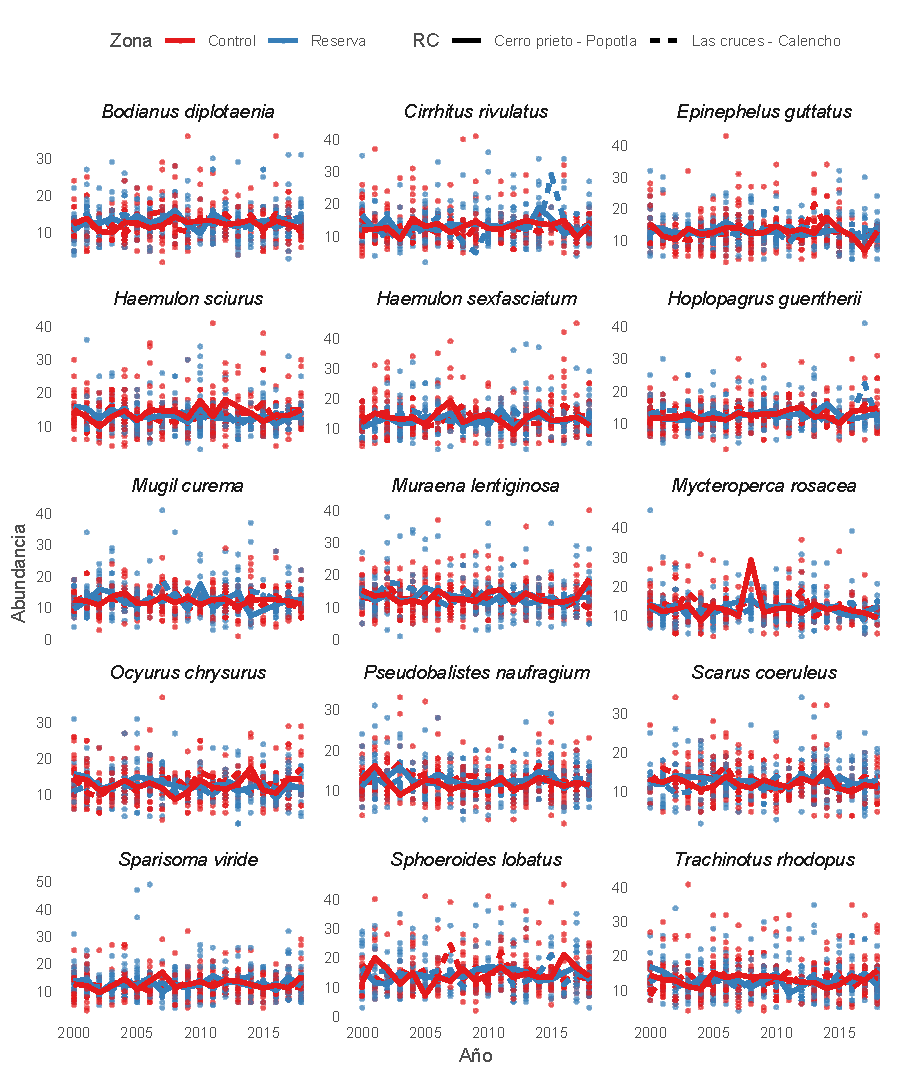
\includegraphics{evaluacion-reservas_files/figure-latex/graficar-datos-1.pdf}
\caption{\label{fig:graficar-datos}Series de tiempo de los datos antes de
agregar tendencias}
\end{figure}

\begin{Shaded}
\begin{Highlighting}[]
\CommentTok{# Ahora agregamos tendencias en abundancias y tallas.}
\CommentTok{# Las abundancias aumentan un 10% cada ano despues del 2000.}
\CommentTok{# Las tallas aumentan 1 cm cada año.}
\NormalTok{datos <-}\StringTok{ }\NormalTok{datos }\OperatorTok
\StringTok{  }\KeywordTok{mutate}\NormalTok{(}\DataTypeTok{neg =} \KeywordTok{ifelse}\NormalTok{(RC }\OperatorTok{==}\StringTok{ "Cerro prieto - Popotla"}\NormalTok{, }\DecValTok{-1}\NormalTok{, }\DecValTok{1}\NormalTok{),}
         \DataTypeTok{Abundancia =} \KeywordTok{ifelse}\NormalTok{(Zona }\OperatorTok{==}\StringTok{ "Reserva"} \OperatorTok{&}\StringTok{ }\NormalTok{Ano }\OperatorTok{>}\StringTok{ }\DecValTok{2000}\NormalTok{,}
\NormalTok{                             Abundancia }\OperatorTok{*}\StringTok{ }\NormalTok{(}\DecValTok{1} \OperatorTok{+}\StringTok{ }\NormalTok{(neg }\OperatorTok{*}\StringTok{ }\NormalTok{((Ano }\OperatorTok{-}\StringTok{ }\DecValTok{2000}\NormalTok{) }\OperatorTok{*}\StringTok{ }\FloatTok{0.1}\NormalTok{))),}
\NormalTok{                             Abundancia),}
         \DataTypeTok{Talla =} \KeywordTok{ifelse}\NormalTok{(Zona }\OperatorTok{==}\StringTok{ "Reserva"} \OperatorTok{&}\StringTok{ }\NormalTok{Ano }\OperatorTok{>}\StringTok{ }\DecValTok{2000}\NormalTok{,}
\NormalTok{                        Talla }\OperatorTok{+}\StringTok{ }\NormalTok{((Ano }\OperatorTok{-}\StringTok{ }\DecValTok{2000}\NormalTok{) }\OperatorTok{*}\StringTok{ }\DecValTok{1}\NormalTok{),}
\NormalTok{                        Talla)) }\OperatorTok\StringTok{ }
\StringTok{  }\KeywordTok{select}\NormalTok{(}\OperatorTok{-}\NormalTok{neg)}
\end{Highlighting}
\end{Shaded}

\begin{Shaded}
\begin{Highlighting}[]
\CommentTok{# Graficar los datos}
\NormalTok{datos }\OperatorTok\StringTok{ }
\StringTok{  }\KeywordTok{ggplot}\NormalTok{(}\KeywordTok{aes}\NormalTok{(}\DataTypeTok{x =}\NormalTok{ Ano, }\DataTypeTok{y =}\NormalTok{ Abundancia, }\DataTypeTok{color =}\NormalTok{ Zona, }\DataTypeTok{group =}\NormalTok{ Sitio, }\DataTypeTok{linetype =}\NormalTok{ RC)) }\OperatorTok{+}
\StringTok{  }\KeywordTok{geom_point}\NormalTok{(}\DataTypeTok{alpha =} \FloatTok{0.5}\NormalTok{, }\DataTypeTok{size =} \FloatTok{0.5}\NormalTok{) }\OperatorTok{+}
\StringTok{  }\KeywordTok{stat_summary}\NormalTok{(}\DataTypeTok{geom =} \StringTok{"line"}\NormalTok{, }\DataTypeTok{fun.y =} \StringTok{"mean"}\NormalTok{, }\DataTypeTok{size =} \DecValTok{1}\NormalTok{) }\OperatorTok{+}
\StringTok{  }\KeywordTok{facet_wrap}\NormalTok{(}\OperatorTok{~}\NormalTok{GeneroEspecie, }\DataTypeTok{ncol =} \DecValTok{3}\NormalTok{, }\DataTypeTok{scales =} \StringTok{"free_y"}\NormalTok{) }\OperatorTok{+}
\StringTok{  }\NormalTok{startR}\OperatorTok{::}\KeywordTok{ggtheme_plot}\NormalTok{() }\OperatorTok{+}
\StringTok{  }\KeywordTok{theme}\NormalTok{(}\DataTypeTok{legend.position =} \StringTok{"top"}\NormalTok{) }\OperatorTok{+}
\StringTok{  }\KeywordTok{scale_color_brewer}\NormalTok{(}\DataTypeTok{palette =} \StringTok{"Set1"}\NormalTok{) }\OperatorTok{+}
\StringTok{  }\KeywordTok{xlab}\NormalTok{(}\StringTok{"Año"}\NormalTok{)}
\end{Highlighting}
\end{Shaded}

\begin{figure}
\centering
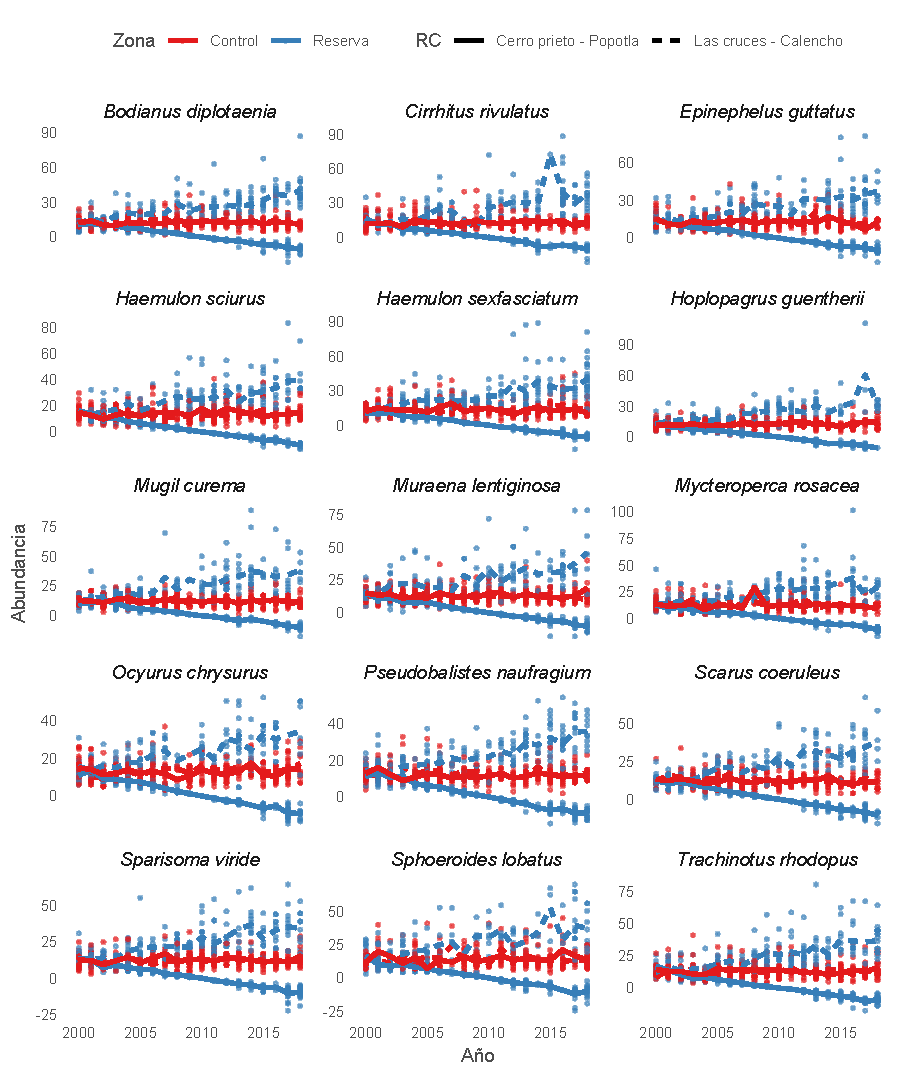
\includegraphics{evaluacion-reservas_files/figure-latex/graficar-datos-abundancias-1.pdf}
\caption{\label{fig:graficar-datos-abundancias}Series de tiempo de los datos
con tendencias (10\% anual) despés del primer año. Note como una reserva
funciona y otra no.}
\end{figure}

\begin{Shaded}
\begin{Highlighting}[]
\CommentTok{# Graficar los datos}
\NormalTok{datos }\OperatorTok\StringTok{ }
\StringTok{  }\KeywordTok{ggplot}\NormalTok{(}\KeywordTok{aes}\NormalTok{(}\DataTypeTok{x =}\NormalTok{ Ano, }\DataTypeTok{y =}\NormalTok{ Talla, }\DataTypeTok{color =}\NormalTok{ Zona, }\DataTypeTok{group =}\NormalTok{ Sitio, }\DataTypeTok{linetype =}\NormalTok{ RC)) }\OperatorTok{+}
\StringTok{  }\KeywordTok{geom_point}\NormalTok{(}\DataTypeTok{alpha =} \FloatTok{0.5}\NormalTok{, }\DataTypeTok{size =} \FloatTok{0.5}\NormalTok{) }\OperatorTok{+}
\StringTok{  }\KeywordTok{stat_summary}\NormalTok{(}\DataTypeTok{geom =} \StringTok{"line"}\NormalTok{, }\DataTypeTok{fun.y =} \StringTok{"mean"}\NormalTok{, }\DataTypeTok{size =} \DecValTok{1}\NormalTok{) }\OperatorTok{+}
\StringTok{  }\KeywordTok{facet_wrap}\NormalTok{(}\OperatorTok{~}\NormalTok{GeneroEspecie, }\DataTypeTok{ncol =} \DecValTok{3}\NormalTok{, }\DataTypeTok{scales =} \StringTok{"free_y"}\NormalTok{) }\OperatorTok{+}
\StringTok{  }\NormalTok{startR}\OperatorTok{::}\KeywordTok{ggtheme_plot}\NormalTok{() }\OperatorTok{+}
\StringTok{  }\KeywordTok{theme}\NormalTok{(}\DataTypeTok{legend.position =} \StringTok{"top"}\NormalTok{) }\OperatorTok{+}
\StringTok{  }\KeywordTok{scale_color_brewer}\NormalTok{(}\DataTypeTok{palette =} \StringTok{"Set1"}\NormalTok{) }\OperatorTok{+}
\StringTok{  }\KeywordTok{xlab}\NormalTok{(}\StringTok{"Año"}\NormalTok{)}
\end{Highlighting}
\end{Shaded}

\begin{figure}
\centering
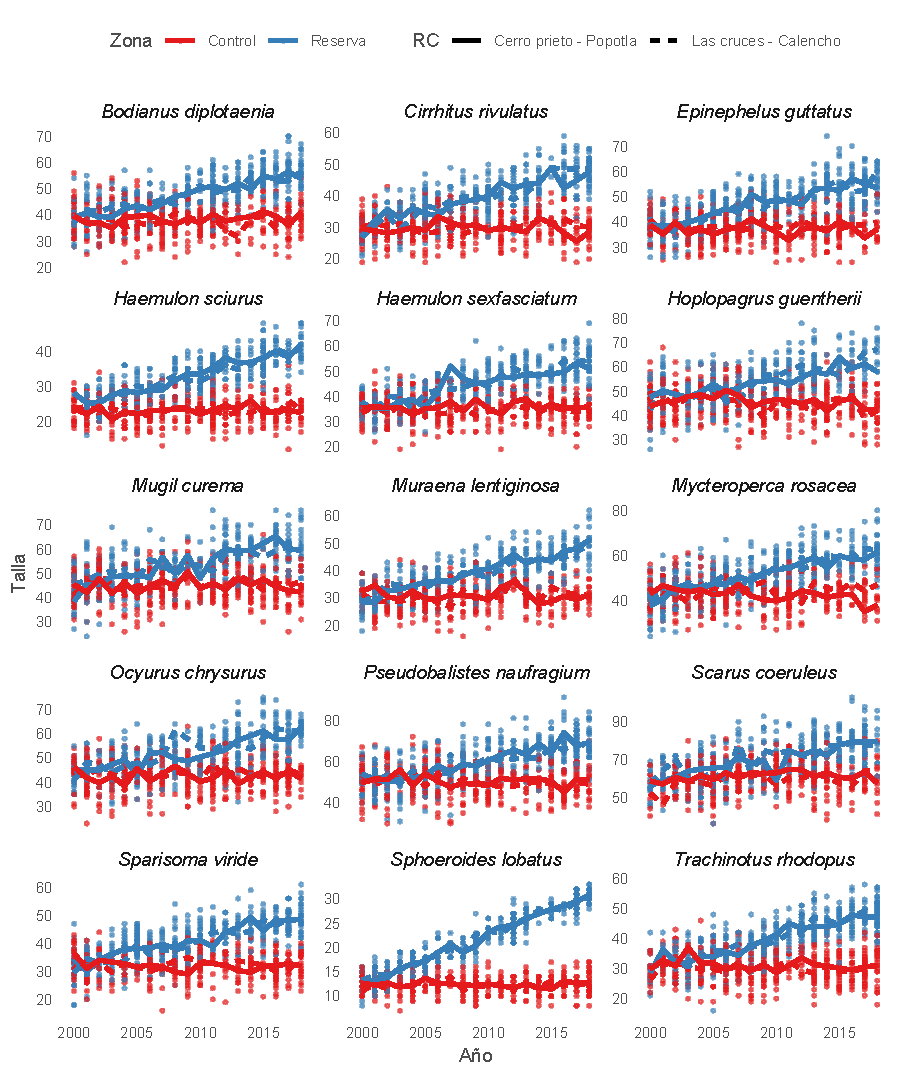
\includegraphics{evaluacion-reservas_files/figure-latex/graficar-datos-tallas-1.pdf}
\caption{\label{fig:graficar-datos-tallas}Series de tiempo de los datos con
tendencias (10\% anual) despés del primer año. Note como una reserva
funciona y otra no.}
\end{figure}

\begin{Shaded}
\begin{Highlighting}[]
\KeywordTok{write.csv}\NormalTok{(}\DataTypeTok{x =}\NormalTok{ datos,}
          \DataTypeTok{file =}\NormalTok{ here}\OperatorTok{::}\KeywordTok{here}\NormalTok{(}\StringTok{"materiales"}\NormalTok{, }\StringTok{"datos"}\NormalTok{, }\StringTok{"datos_peces.csv"}\NormalTok{),}
          \DataTypeTok{row.names =}\NormalTok{ F)}
\end{Highlighting}
\end{Shaded}

\bibliography{references.bib}

\backmatter
\printindex

\end{document}
